\textbf{Ejemplo 6}\\

\vspace{2mm}
Para la compra de un automóvil que vale 6.000.000 COP; se exige una cuota inicial del 40\% y el resto se cancela en 36 cuotas mensuales, ¿a cuánto ascenderá la cuota, si lo intereses son del 2\% período mes vencido?\\ \\
%\newpage %USAR SOLO SI EL SOLUCIÓN QUEDA SOLO Y ES NECESARIO BAJARLO A LA SIGUIENTE PAGINA
\textbf{Solución.}
%La tabla ira centrada
\begin{center}
 \renewcommand{\arraystretch}{1.5}% Margenes de las celdas
 %Creación de la cuadricula de 3 columnas
 \begin{longtable}[H]{|p{0.333\linewidth}|p{0.3333\linewidth}|p{0.3333\linewidth}|}
  \hline
  \multicolumn{3}{|c|}{\cellcolor[HTML]{FFB183}\textbf{1. Declaración de variables}}             \\ \hline
  $VP= 6.000.000 COP $     & $i=2\% \hspace{1mm} pmv$                  & $R =   ? COP$            \\
  $n=36 \hspace{1mm} pmv$ & $\text{Cuota inicial}=40\% \hspace{1mm} VP$ &                        \\ \hline
  \multicolumn{3}{|c|}{\cellcolor[HTML]{FFB183}\textbf{2. Tabla de flujo de caja}}               \\ \hline
  \multicolumn{3}{|p{\columnwidth}|}{
  \begin{center}
   \begin{tabular}{ |p{3.5cm}| p{3cm}|}
    \hline
    \textbf{Periodo (psv) } & \textbf{Flujo} \\ \hline
    0                       & -              \\\hline
    1                       &  COP ?            \\ \hline
    2                       &  COP ?            \\ \hline
    3                       &  COP ?            \\ \hline
    4                       &  COP ?            \\ \hline
    5                       &  COP ?            \\ \hline
    6                       &  COP ?            \\ \hline
    7                       &  COP ?            \\ \hline
    8                       &  COP ?            \\ \hline
    9                       &  COP ?            \\ \hline
    10                      &  COP ?            \\ \hline
    11                      &  COP ?            \\ \hline
    12                      &  COP ?            \\ \hline
    13                      &  COP ?            \\ \hline
    14                      &  COP ?            \\ \hline
    15                      &  COP ?            \\ \hline
    16                      &  COP ?            \\ \hline
    17                      &  COP ?            \\ \hline
    18                      &  COP ?            \\ \hline
    19                      &  COP ?            \\ \hline
    20                      &  COP ?            \\ \hline
    21                      &  COP ?            \\ \hline
    22                      &  COP ?            \\ \hline
    23                      &  COP ?            \\ \hline
    24                      &  COP ?            \\ \hline
    25                      &  COP ?            \\ \hline
    26                      &  COP ?            \\ \hline
    27                      &  COP ?            \\ \hline
    28                      &  COP ?            \\ \hline
    29                      &  COP ?            \\ \hline
    30                      &  COP ?            \\ \hline
    31                      &  COP ?            \\ \hline
    32                      &  COP ?            \\ \hline
    33                      &  COP ?            \\ \hline
    34                      &  COP ?            \\ \hline
    35                      &  COP ?            \\ \hline
    36                      &  COP ?            \\ \hline
   \end{tabular}
  \end{center}
  }                                                                                              \\ \hline
  \multicolumn{3}{|c|}{\cellcolor[HTML]{FFB183}\textbf{3. Fórmulas utilizadas}}                  \\ \hline
  \multicolumn{3}{|p{\columnwidth}|}{Mediante el uso de Excel:
  \begin{itemize}
   \item PAGO: Calcula el pago de un préstamo, basado en los pagos y tasa de interés
         constantes.
  \end{itemize}
  }                                                                                              \\ \hline
  \multicolumn{3}{|c|}{\cellcolor[HTML]{FFB183}\textbf{4. Desarrollo en Excel}}                  \\ \hline
  \multicolumn{3}{|p{\columnwidth}|}{
  Se aplicará la función PAGO de la siguiente forma:

  =PAGO(0,06;5;-3000000) con referencia en la hoja de Excel usada para el ejercicio.
  }                                                                                              \\
  \multicolumn{3}{|c|}{ 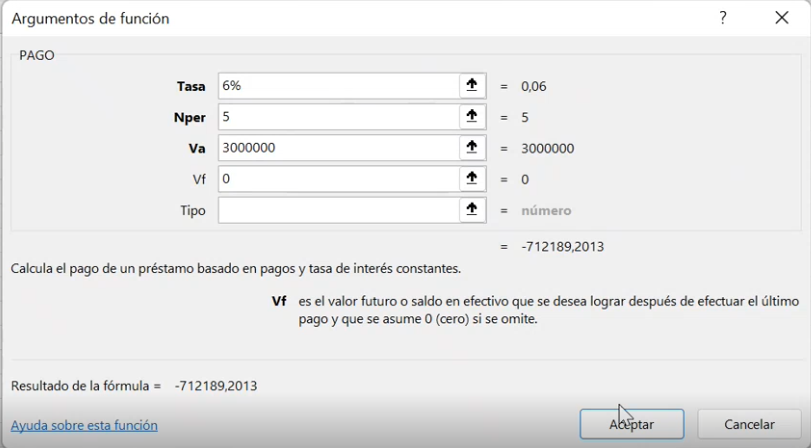
\includegraphics[trim=-5 -5 -5 -5 ,width=1\columnwidth]{6/Ejem6.png}}    \\
  \multicolumn{3}{|c|}{\cellcolor[HTML]{FFB183}\textbf{5. Respuesta}}                            \\ \hline
  \multicolumn{3}{|p{\columnwidth}|}{
  La cuota ascenderá a   712.189 COP
  }                                                                                              \\ \hline
  \multicolumn{3}{|c|}{\cellcolor[HTML]{FFB183}\textbf{6. Gráfica}}                              \\ \hline
  \multicolumn{3}{|c|}{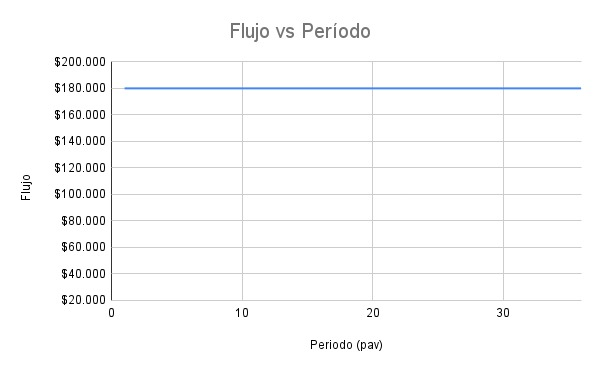
\includegraphics[trim=-5 -5 -5 -5 ,width=0.7\columnwidth]{6/flujovsperiodo6.png}} \\ \hline
 \end{longtable}
 %\newline \newline %USARLO SI CREES QUE ES NECESARIO
\end{center}
